Some features might be more expressive than others, and finding the set of features that will yield the best result is imperative. The test on the cluster is performed with logistic regression using stochastic gradient descent and L2 regularization with a ridge value of 0.01. 
For each feature test 1348428 games is used for training and 577552 games are used for evaluation. 
The feature sets tested are:
\begin{itemize}
\item blue team, purple team 
\item blue combos, purple combos
\item blue team, purple team, blue combos, purple combos
\item blue team, purple team, blue combos, purple combos, cross team combos
\item blue team, purple team, blue combos, purple combos, cross team combos, champion ranks
\item all features 
\end{itemize}

% Graph for feature testing. 
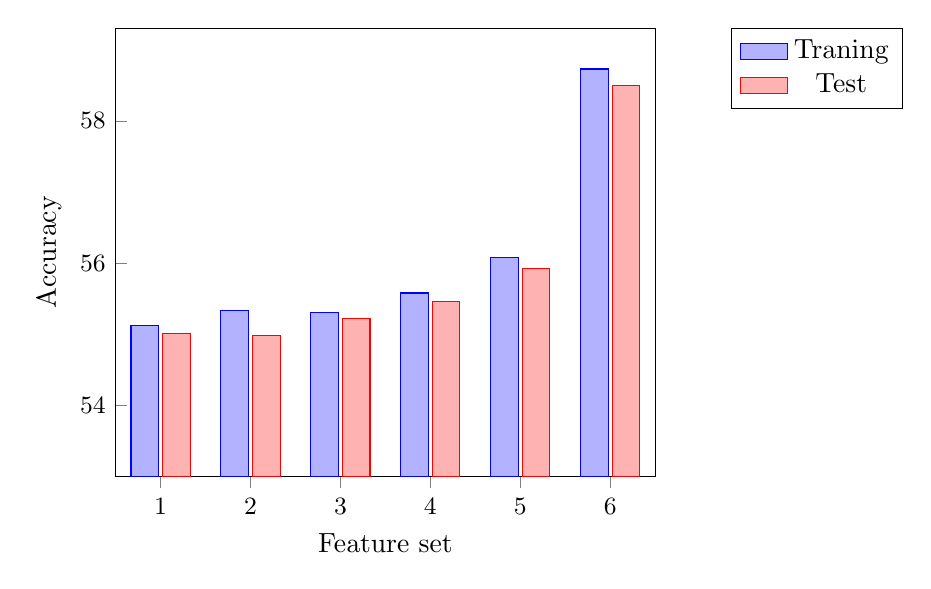
\begin{tikzpicture}
\begin{axis}[
    ybar,
    ylabel = Accuracy,
    xlabel = Feature set,
    tick label style={font=\small},
    tickpos=left,
    xticklabels={1, 2, 3, 4, 5, 6}, 
    xtick={1,2,3,4,5, 6},
    ymin=53,
    legend entries={Traning,Test},
    legend style={at={(1.3,1.0)},
        anchor=north,legend columns=1
    },
    legend image code/.code={%
      \draw[#1] (0cm,-0.1cm) rectangle (0.6cm,0.1cm);
    }   
    ]   
    \addplot +[bar shift=-.2cm] coordinates {(1,55.12) (2,55.34) (3,55.31)  (4,55.58)     (5,56.08)  (6, 58.73)};

    \addplot  +[bar shift=.2cm]coordinates {(1,55.01) (2,54.98) (3,55.22) (4,  55.46) (5,55.92) (6, 58.50)};

\end{axis}
\end{tikzpicture}


% Graph for big data testing. 
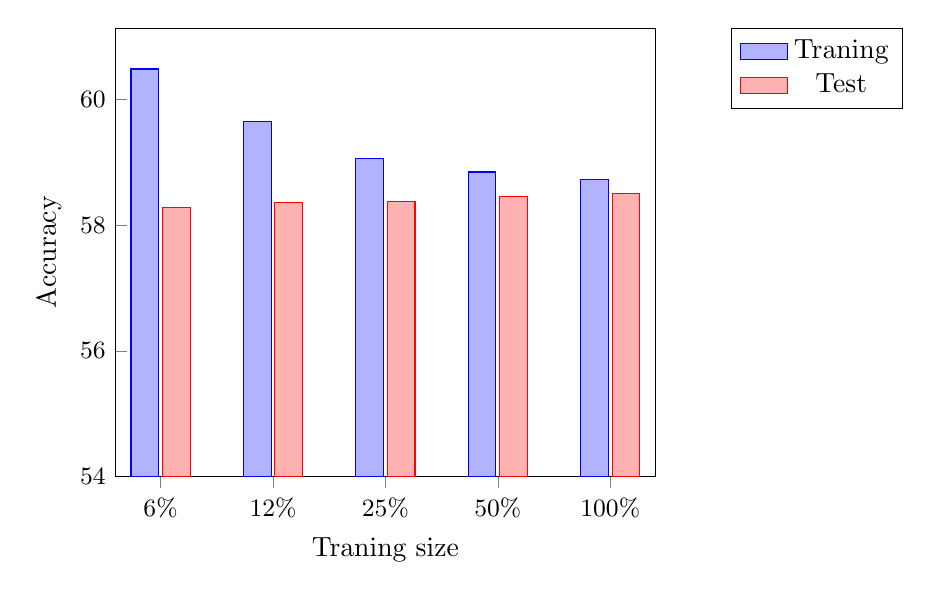
\begin{tikzpicture}
\begin{axis}[
    ybar,
    ylabel = Accuracy,
    xlabel = Traning size,
    tick label style={font=\small},
    tickpos=left,
    xticklabels={6\%, 12\%, 25\%, 50\%, 100\%}, 
    xtick={1,2,3,4,5, 6},
    ymin=54,
    legend entries={Traning,Test},
    legend style={at={(1.3,1.0)},
        anchor=north,legend columns=1
    },
    legend image code/.code={%
      \draw[#1] (0cm,-0.1cm) rectangle (0.6cm,0.1cm);
    }   
    ]   
    \addplot +[bar shift=-.2cm] coordinates {(1,60.49) (2,59.66) (3,59.06)  (4,58.85)     (5,58.73)  };

    \addplot  +[bar shift=.2cm]coordinates {(1,58.28) (2,58.36) (3,58.38) (4,  58.46) (5,58.50) };

\end{axis}
\end{tikzpicture}